\subsection{Scénario Cockburn}
\textbf{Cas d'utilisation: Payer par Télépéage}

\textbf{Acteur primaire:} Le conducteur

%\textbf{Acteur support:}

\textbf{Pré-condition: }  La borne est une borne télépéage ou mixte
 
%\textbf{Post-condition: } 

\textbf{Scenario primaire: } \\
    \textbf{1.} La borne détecte le badge télépéage\\
    \textbf{2.} La borne enregistre le passage dans l’ordinateur central.\\

\textbf{Variantes:}\\
    \textbf{1a.} La borne ne détecte pas le badge. un technicien est appellé.\\
   \textbf{2a.} La borne n’ouvre pas la barrière. Le conducteur appelle le technicien.\\



%\subsection{{Décomposition des cas d'utilisation:} 
%\begin{figure}[h]
 %   \centering
  %  \includegraphics[scale=0.7]{02_Desenvolvimento/TD2/images/PaiementTelepeage.png}
   % \caption{Décomposition des cas d'utilisation: Payer avec abonnement Télépéage}
%\end{figure}
\newpage
\subsection{Diagramme d'activité}
\begin{figure}[h]
    \centering
    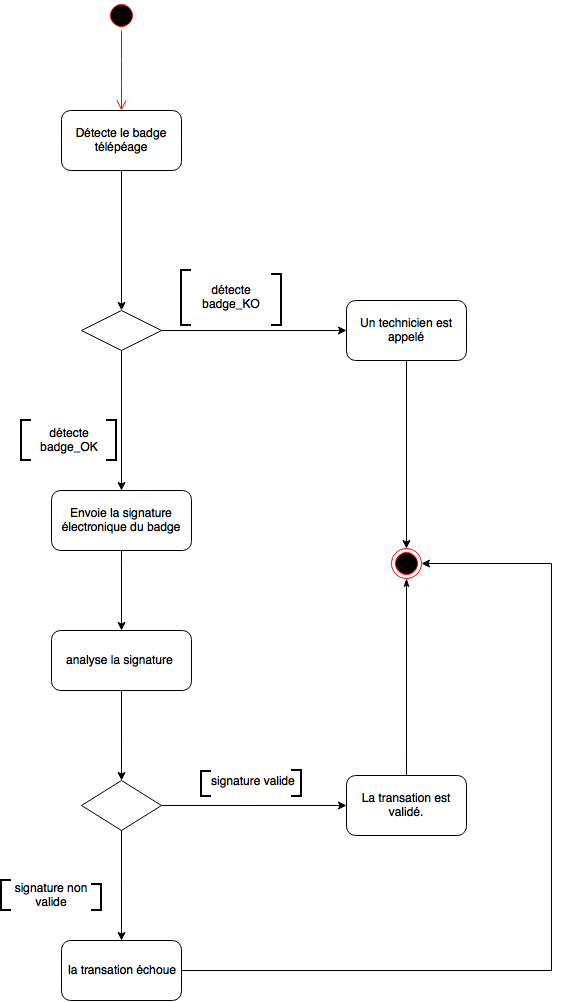
\includegraphics[scale=0.7]{02_Desenvolvimento/TD2/images/DATelepeage.png}
    \caption{Diagramme d'activité: Payer par Telépéage}
\end{figure}
\newpage
\subsection{Collaboration}
\begin{figure}[h]
    \centering
    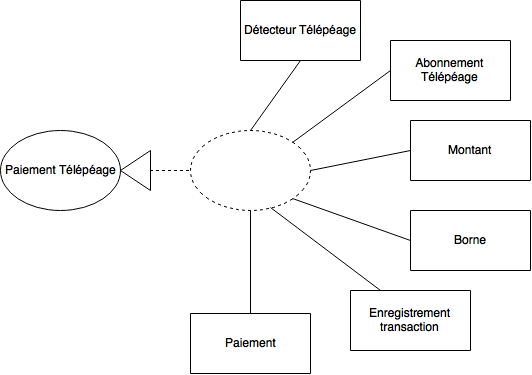
\includegraphics[scale=0.6]{02_Desenvolvimento/TD2/images/ColaTelepeage.png}
    \caption{Collaboration: Payer par Telépéage}
\end{figure}
